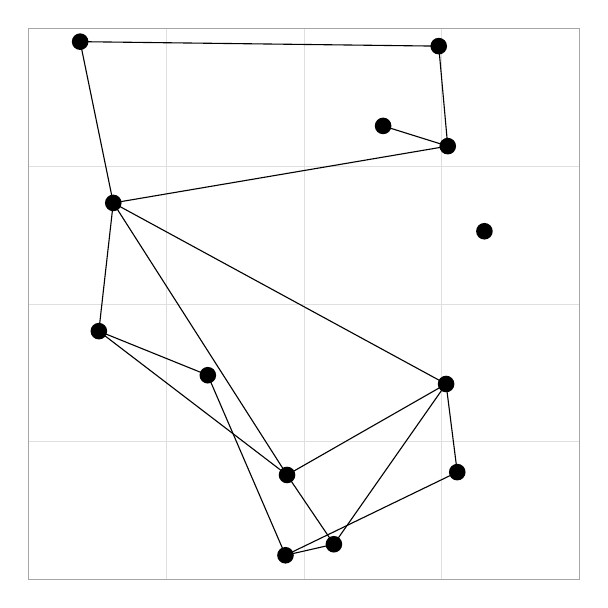
\begin{tikzpicture}[x=1.75cm, y=1.75cm]
% Generated by scripts/generate_sirg.py: seed=42, vertices=13, process=cox(period=2, phase=(1.54791,0.877757)), line width=0.4pt, opacity=1
% Ambient window
\draw[step=1, very thin, gray!25]
    (-2,-2) grid (2,2);
\draw[thin, gray!70]
    (-2,-2) rectangle (2,2);

% Vertices
\coordinate (v0) at (-1.6232906,1.9024894);
\coordinate (v1) at (1.0445588,1.1442572);
\coordinate (v2) at (-1.4875455,-0.19845625);
\coordinate (v3) at (0.57546048,1.2910465);
\coordinate (v4) at (0.21833915,-1.744731);
\coordinate (v5) at (1.3105247,0.5266576);
\coordinate (v6) at (1.032351,-0.58189613);
\coordinate (v7) at (1.113534,-1.2214452);
\coordinate (v8) at (-0.13311599,-1.8247849);
\coordinate (v9) at (-1.382842,0.73219581);
\coordinate (v10) at (0.97904862,1.8700389);
\coordinate (v11) at (-0.69669857,-0.51816118);
\coordinate (v12) at (-0.12177675,-1.2421146);

% Edges
\draw[line width=0.4pt, opacity=1] (v0) -- (v9);
\draw[line width=0.4pt, opacity=1] (v0) -- (v10);
\draw[line width=0.4pt, opacity=1] (v1) -- (v3);
\draw[line width=0.4pt, opacity=1] (v1) -- (v9);
\draw[line width=0.4pt, opacity=1] (v1) -- (v10);
\draw[line width=0.4pt, opacity=1] (v2) -- (v9);
\draw[line width=0.4pt, opacity=1] (v2) -- (v11);
\draw[line width=0.4pt, opacity=1] (v2) -- (v12);
\draw[line width=0.4pt, opacity=1] (v4) -- (v6);
\draw[line width=0.4pt, opacity=1] (v4) -- (v8);
\draw[line width=0.4pt, opacity=1] (v4) -- (v12);
\draw[line width=0.4pt, opacity=1] (v6) -- (v7);
\draw[line width=0.4pt, opacity=1] (v6) -- (v9);
\draw[line width=0.4pt, opacity=1] (v6) -- (v12);
\draw[line width=0.4pt, opacity=1] (v7) -- (v8);
\draw[line width=0.4pt, opacity=1] (v8) -- (v11);
\draw[line width=0.4pt, opacity=1] (v9) -- (v12);

% Vertices
\foreach \v in {v0,v1,v2,v3,v4,v5,v6,v7,v8,v9,v10,v11,v12} {
    \fill (\v) circle (3pt);
}
\end{tikzpicture}
